\section{Conclusion}

\begin{figure}[b]
	\vspace{2mm}
\centerline{%
	\subfigure[scale]{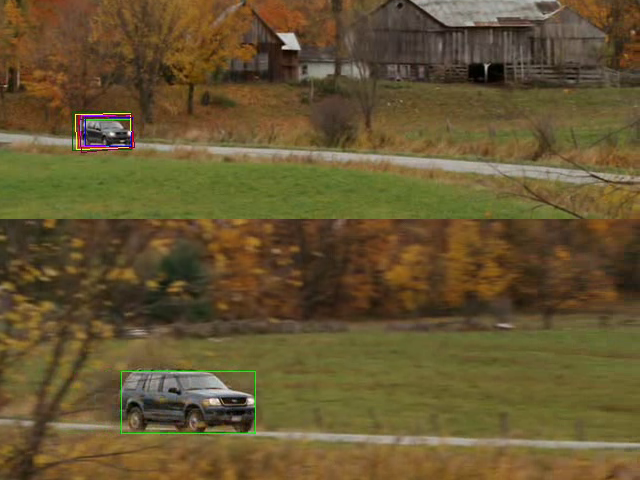
\includegraphics[width=0.33\linewidth]{imgs/limitations/scale.png}\label{fig:tra}}
	\subfigure[light]{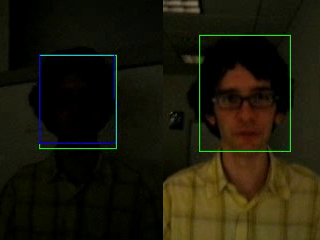
\includegraphics[width=0.33\linewidth]{imgs/limitations/light.png}\label{fig:trb}}
	\subfigure[multi-instance]{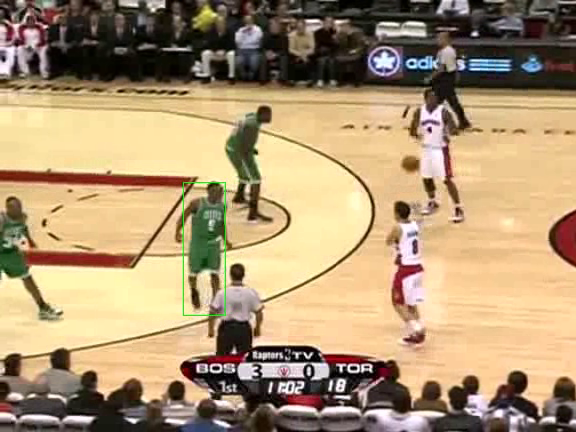
\includegraphics[width=0.33\linewidth]{imgs/limitations/basket.png}\label{fig:trc}}}
	\vspace{-2mm}
\caption{Examples showing the main problems that feature descriptors cannot address. }
\label{fig:tracking_results_scale}
\end{figure} 



We proposed an evaluation of the most common feature descriptors for the purpose of tracking by detection. Our experiments have shown that most of the feature descriptors have comparable results. While AKAZE and SIFT have proven to be more distinctive, ORB and BRISK compensate their weak descriptors with a higher number of points extracted. Given the growing interested in AKAZE descriptor we provided a GPU implementation so that it can be used for real time system. The code to perform the benchmark, the dataset and our implementation of AKAZE will be publicly available in order to ease researches in this area.



\begin{table*}[h]
\caption{Tracking results with low,medium and high accuracy requirements. The high number of key points extracted by ORB or BRISK compensate their weak descriptors. This comes with a cost in performance.} 
\centerline{%
		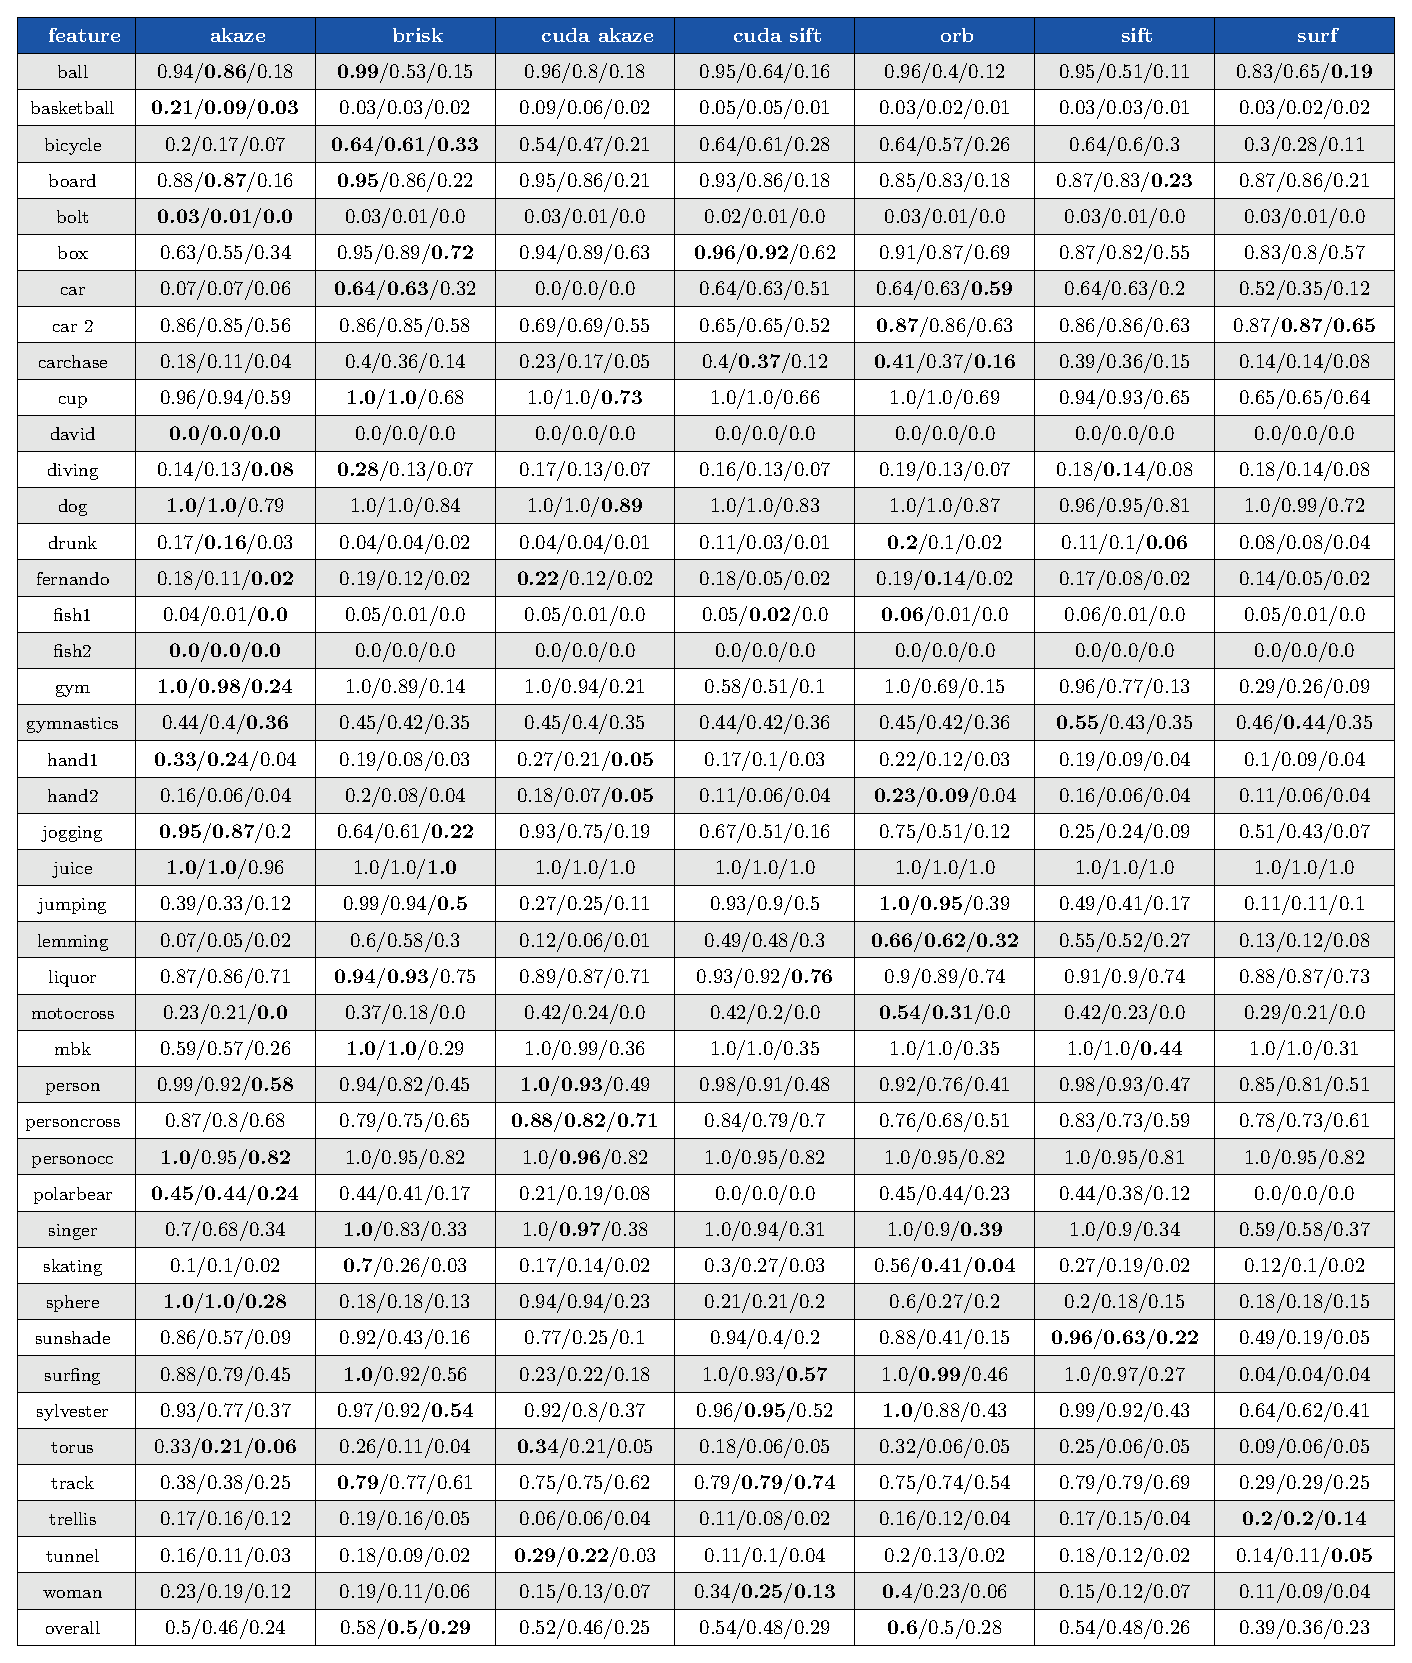
\includegraphics[width=0.98\linewidth]{tables/tracking_precision.pdf}}
    \vspace{-2mm} 
	\label{table:taccuracy}
\end{table*}